\documentclass[12pt]{article}
\usepackage{amsmath}
\usepackage{tikz}
\usepackage{graphicx}
\graphicspath{ {./images/} }
\begin{document}
\title{Statics Review}
\author{Aditya Dangra}
\date{\today}
\maketitle

\pagenumbering{roman}
\tableofcontents
\pagebreak
\pagenumbering{arabic}

\section{Chapter 1: General Principles}
Statics deals with the equilibrium of bodies, that is, those that are at rest or moving with constant velocity.
Its importance to the real world stems from the need to keep things from moving, such as buildings or bridges.

\subsection{Important Points}
The following points outline the foundations upon which the study of Statics is built upon.
\begin{itemize}
    \item Statics is the study of bodies that are at rest or moving with constant velocity \cite{hibbeler}.
    \item Newton's three laws of motion are integral to the study of statics and should be memorized.
    \item If size is negligible, then a system can be reduced to a single particle containing all of its mass.
    \item Concentrated forces are assumed to act at a single point on a body (In reality, all forces are distributed loads).
    \item The meter, second, and kilogram are base units of the SI system.
    \item The foot, second, and pound are base units of the Imperial system.
    \item Mass measures the quantity of matter that does not change depending on location. Weight refers to the gravitational attraction of the earth on a quantity of mass.
\end{itemize}

\subsection{General Procedure}
Attending lectures, reading books, and studying example problems help, but \textbf{the most effective way of learning is to \textit{solve problems}} \cite{hibbeler}.
The following is a generalized procedure that should apply to all problems and ensure success:
\begin{itemize}
    \item Read the problem and try to correlate the situation with the theory studied.
    \item Draw a free body diagram of the situation with all necessary forces, moments, and dimensions.
    \item Write out any relavent equations and diagrams.
    \item Solve the necessary equations in an effecient manner.
    \item Study the answer with technical judgement and common sense to determine whether it seems reasonable.
\end{itemize}

\subsection{Relavent Problems}
In Chapter 1, the problems focus on unit conversions and Newton's Law of Gravitation.
Some relavent problems include:
\begin{itemize}
    \item Unit Conversions:
    \begin{itemize}
        \item 1-2, 1-7, 1-9, 1-10, 1-14
    \end{itemize}
    \item Density and Gravitation:
    \begin{itemize}
        \item 1-17, 1-19, 1-21
    \end{itemize}
\end{itemize}

\pagebreak
\section{Chapter 2: Force Vectors}
A \textbf{scalar} is any positive or negative quantity that can be specified by its \textit{magnitude}.
A \textbf{vector} is any quantity that requires both a \textit{magnitude} and a \textit{direction} \cite{buckham}.
A vector is shown graphically by an arrow indicating the sense of direction and an angle $\theta$ between the vector and a fixed axis.

\subsection{Vector Operations}
Like scalars, vectors can also be added and multiplied, but a slightly different set of rules apply.

\subsubsection*{Multiplication by a Scalar}
When a vector is multiplied by a scalar, its magnitude will be increased by that amount. 
Multiplying by a negative reverses the direction of the vector.

\subsubsection*{Vector Addition}
Adding vectors is done \textit{tip to tail}, as in the second vector's tail is moved to the tip of the first vector (Figure 1).
The vector between the first tail and the final tip is the \textbf{resultant}, another vector.
Vectors can also be added component-wise, where the $x$-component of the resultant is the sum of the $x$-components of the vectors being added and so on.

\begin{figure}
\centering
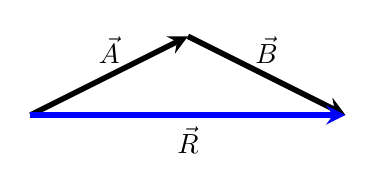
\begin{tikzpicture}
    \draw[line width=2pt, black, -stealth](0, 0) -- (2, 1) node[midway, above]{$\vec{A}$};
    \draw[line width=2pt, black, -stealth](2, 1) -- (4, 0) node[midway, above]{$\vec{B}$};
    \draw[line width=2pt, blue, -stealth](0, 0) -- (4, 0) node[midway, below, text=black]{$\vec{R}$};
\end{tikzpicture}
\caption{Adding two vectors \textit{tip to tail}}
\end{figure}

\subsubsection*{Vector Subtraction}
Vector subtraction is defined as a special case of vector addition.
Instead of being subtracted, the vector is multiplied by $-1$ and instead added (shown below).

\begin{equation*}
    \vec{R} = \vec{A} - \vec{B} = \vec{A} + \left(-\vec{B}\right)
\end{equation*}

\subsection{Force Components}
Forces can be represented with magnitude and direction but it is usually easier to work with components in the $x$, $y$, and $z$ directions.
It is possible to calculate the components using an angle and magnitude or with the \textbf{coordinate direction angles} $\alpha$ (alpha), $\beta$ (beta), and $\gamma$ (gamma).
Coordinate direction angles are measured between the vector and the \textit{positive} $x$, $y$, and $z$ axes.
$\alpha$, $\beta$, and $\gamma$ for a vector $\vec{A}$ are defined as:
\begin{align*}
    \cos{\alpha} &= \frac{A_x}{A} & \cos{\beta} &= \frac{A_y}{A} & \cos{\gamma} &= \frac{A_z}{A} \\
\end{align*}
The following identity also holds:
\begin{equation*}
    \cos^2{\alpha} + \cos^2{\beta} + cos^2{\gamma} = 1
\end{equation*}
Sometimes, the direction of a vector can be specified in terms of a \textbf{transverse angle} $\theta$ and an \textbf{azmuth angle} $\phi$, as shown in figure 2.
The formula to find the components should not be memorized, instead determined by trigonometry.
\begin{figure}[h]
\centering
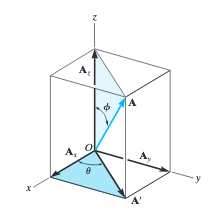
\includegraphics[scale=0.7]{transverse_azmuth.png}
\caption{A vector's direction in terms of $\theta$ and $\phi$ \cite{hibbeler}}
\end{figure}
\pagebreak

\subsection{The Dot Product}
The dot product can be used to find the angle between 2 vectors.
Expressed in equation form:
\begin{align*}
    \vec{A}\cdot\vec{B} &= \left|\vec{A}\right|\left|\vec{B}\right|\cos{\theta} \\
                        &= A_xB_x + A_yB_y + A_zB_z
\end{align*}
The magnitude of the projection of $\vec{A}$ onto $\vec{u_a}$ is determined from the dot product, $A_a = \vec{A}\cdot\vec{u_a}$.



\pagebreak
\addcontentsline{toc}{section}{References}
\begin{thebibliography}{2}
    \bibitem{hibbeler}
    R. C. Hibbeler, \textit{Engineering Mechanics: Statics \& Dynamics (Fourteenth Edition)}, Pearson Prentice Hall, Hoboken, New Jersey, 2016.
    \bibitem{buckham}
    B. Buckham, \textit{ENGR 141 Lecture}, University of Victoria, Victoria, B.C., 2019.
\end{thebibliography}

\end{document}